\documentclass[11pt,letterpaper]{article}
\usepackage[lmargin=1in,rmargin=1in,tmargin=1in,bmargin=1in]{geometry}
\usepackage{../style/homework}
\usepackage{../style/commands}
\setbool{quotetype}{true} % True: Side; False: Under
\setbool{hideans}{true} % Student: True; Instructor: False

% -------------------
% Content
% -------------------
\begin{document}

\homework{2: Due 09/13}{Science is simply common sense at its best; that is, rigidly accurate in observation, and merciless to fallacy in logic.}{Thomas Huxley}

% Problem 1
\problem{10} Show that $P \wedge (\neg Q \vee R) \to (P \wedge R) \vee \neg Q$ is a tautology by constructing its truth table. Using words, explain why this expression is a tautology without making reference to its truth table.



\newpage



% Problem 2
\problem{10} Consider the statement, ``If $n$ is even, then $n$ is not prime or $n$ is 2.''
	\begin{enumerate}[(a)]
	\item By defining appropriate propositions, write the given statement as a logical expression.
	\item Write the converse of your answer in (a). Then write this logical expression in words. Is this statement true? Explain.
	\item Write the contrapositive of your answer in (a). Then write this logical expression in words. Is this statement true? Explain. 
	\end{enumerate}



\newpage



% Problem 3
\problem{10} Suppose the statement, ``If this metal is glowing red, then its temperature must be at least 460$^\circ$C,'' is true. Indicate whether the following statements are true or false. No justification is necessary.
	\begin{enumerate}[(a)]
	\item If the temperate of the metal is at least 460$^\circ$C, then it is glowing red.
	\item If the temperature of the metal is less than 460$^\circ$C, then it is not glowing red.
	\item The metal will only glow red if its temperature is at least 460$^\circ$C.
	\item If the metal is now glowing red, then its temperature is less than 460$^\circ$C.
	\item A necessary condition for the metal to glow red is that its temperature be at least 460$^\circ$C.
	\item A sufficient condition for the metal to glow red is that its temperature is at least 460$^\circ$C.
	\end{enumerate}



\newpage



% Problem 4
\problem{10} Suppose one defines a logical connective `$\boxplus$' by saying that $P \boxplus Q$ is true if and only if \textit{both} $P$ and $Q$ are true.
	\begin{enumerate}[(a)]
	\item Construct the truth table for $P \boxplus Q$.
	\item Using a truth table, show that $(P \boxplus Q) \equiv (P \leftrightarrow Q) \wedge P$ and $(P \boxplus Q) \equiv (P \leftrightarrow Q) \wedge Q$.
	\item Without referencing a truth table, explain the logical equivalences in (b).
	\item Using the result from (b)---but without referencing a truth table---explain why $\big( (P \boxplus Q) \big) \leftrightarrow \big( (P \leftrightarrow Q) \wedge P \big)$ and $\big( (P \boxplus Q) \big) \leftrightarrow \big( (P \leftrightarrow Q) \wedge P \big)$ are tautologies. 
	\item Without using a truth table, explain why $P \boxplus Q \equiv Q \boxplus P$.
	\end{enumerate}



\newpage



% Problem 5
\problem{10} Find a Boolean expression that represents the following circuit and construct its input/output table.
	\begin{figure}[!ht]
	\centering
	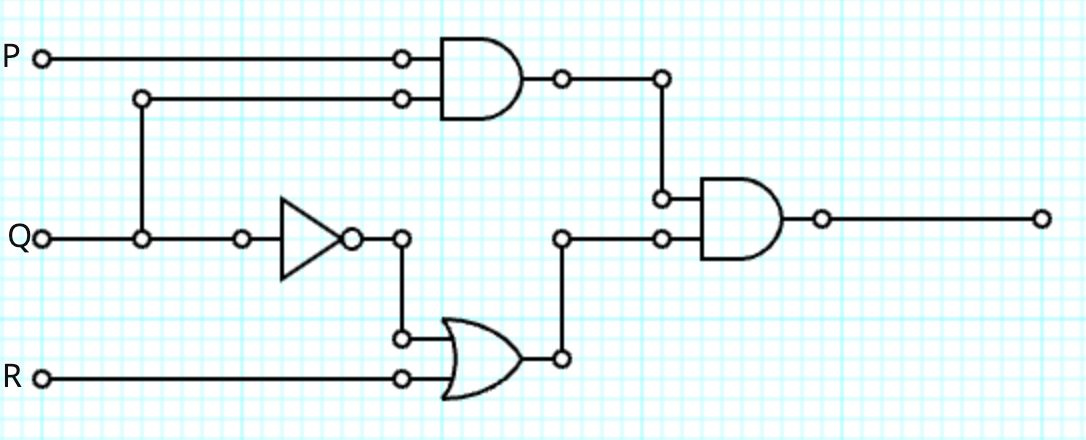
\includegraphics[width=0.75\textwidth]{circuit.png}
	\end{figure} 



\newpage



% Problem 6
\problem{10} Draw a circuit diagram corresponding to the Boolean expression $\neg (P \vee Q) \wedge Q$. 



\newpage



% Problem 7
\problem{10} Suppose a certain tax exemption applies to individuals that make less than than \$55,000 a year, or have three dependents and have at least \$6,000 in charitable donations. Define appropriate propositions and write the condition for this tax exemption as a Boolean expression. Then construct a circuit diagram corresponding to this Boolean expression. 



\newpage



% Problem 8
\problem{10} Watch at least one of the following videos:
	\begin{itemize}
	\item \href{https://www.youtube.com/watch?v=QZwneRb-zqA&ab_channel=SebastianLague}{Exploring How Computers Work}
	\item \href{https://www.youtube.com/watch?v=I0-izyq6q5s&ab_channel=SebastianLague}{How Do Computers Remember?}
	\end{itemize}
Then as thoroughly as possible, comment on what you observed and learned from the video. Be sure to remark as much as possible on how these videos connect to the course content. 









\end{document}